
\documentclass[11pt,a4paper]{report}%especifica o tipo de documento que tenciona escrever: carta, artigo, relatório... neste caso é um relatório
% [11pt,a4paper] Define o tamanho principal das letras do documento. caso não especifique uma delas, é assumido 10pt
% a4paper -- Define o tamanho do papel.

\usepackage[portuges]{babel}%Babel -- irá activar automaticamente as regras apropriadas de hifenização para a língua todo o
                                   %-- o texto gerado é automaticamente traduzido para Português.
                                   %  Por exemplo, “chapter” irá passar a “capítulo”, “table of contents” a “conteúdo”.
                                   % portuges -- específica para o Português.
\usepackage[utf8]{inputenc} % define o encoding usado texto fonte (input)--usual "utf8" ou "latin1

\usepackage{graphicx} %permite incluir graficos, tabelas, figuras
\usepackage{url} % para utilizar o comando \url{}
\usepackage{enumerate} %permite escolher, nas listas enumeradas, se os iems sao marcados com letras ou numeros-romanos em vez de numeracao normal

%\usepackage{apalike} % gerar biliografia no estilo 'named' (apalike)

\usepackage{color} % Para escrever em cores
\usepackage{xcolor}

\usepackage{multirow} %tabelas com multilinhas
\usepackage{array} %formatação especial de tabelas em array

\usepackage[pdftex]{hyperref} % transformar as referências internas do seu documento em hiper-ligações.

% Para autómatos
\usepackage{tikz}
\usetikzlibrary{automata,arrows,positioning, arrows.meta, shapes.geometric}

\usepackage{amsmath,amssymb,amsfonts}
\usepackage{pdfpages}
\usepackage{float} % Image location specifier

%Exemplos de fontes -- nao e vulgar mudar o tipo de fonte
%\usepackage{tgbonum} % Fonte de letra: TEX Gyre Bonum
%\usepackage{lmodern} % Fonte de letra: Latin Modern Sans Serif
%\usepackage{helvet}  % Fonte de letra: Helvetica
%\usepackage{charter} % Fonte de letra:Charter

\definecolor{saddlebrown}{rgb}{0.55, 0.27, 0.07} % para definir uma nova cor, neste caso 'saddlebrown'

\usepackage{listings}  % para utilizar blocos de texto verbatim no estilo 'listings'
%paramerização mais vulgar dos blocos LISTING - GENERAL

%
%\lstset{ %
%	language=Java,							% choose the language of the code
%	basicstyle=\ttfamily\footnotesize,		% the size of the fonts that are used for the code
%	keywordstyle=\bfseries,					% set the keyword style
%	%numbers=left,							% where to put the line-numbers
%	numberstyle=\scriptsize,				% the size of the fonts that are used for the line-numbers
%	stepnumber=2,							% the step between two line-numbers. If it's 1 each line
%											% will be numbered
%	numbersep=5pt,							% how far the line-numbers are from the code
%	backgroundcolor=\color{white},			% choose the background color. You must add \usepackage{color}
%	showspaces=false,						% show spaces adding particular underscores
%	showstringspaces=false,					% underline spaces within strings
%	showtabs=false,							% show tabs within strings adding particular underscores
%	frame=none,								% adds a frame around the code
%	%abovecaptionskip=-.8em,
%	%belowcaptionskip=.7em,
%	tabsize=2,								% sets default tabsize to 2 spaces
%	captionpos=b,							% sets the caption-position to bottom
%	breaklines=true,						% sets automatic line breaking
%	breakatwhitespace=false,				% sets if automatic breaks should only happen at whitespace
%	title=\lstname,							% show the filename of files included with \lstinputlisting;
%											% also try caption instead of title
%	escapeinside={\%*}{*)},					% if you want to add a comment within your code
%	morekeywords={*,...}					% if you want to add more keywords to the set
%}

\usepackage{xspace} % deteta se a seguir a palavra tem uma palavra ou um sinal de pontuaçao se tiver uma palavra da espaço, se for um sinal de pontuaçao nao da espaço

\parindent=0pt %espaço a deixar para fazer a  indentação da primeira linha após um parágrafo
\parskip=2pt % espaço entre o parágrafo e o texto anterior

\setlength{\oddsidemargin}{-1cm} %espaço entre o texto e a margem
\setlength{\textwidth}{18cm} %Comprimento do texto na pagina
\setlength{\headsep}{-1cm} %espaço entre o texto e o cabeçalho
\setlength{\textheight}{23cm} %altura do texto na pagina

% comando '\def' usado para definir abreviatura (macros)
% o primeiro argumento é o nome do novo comando e o segundo entre chavetas é o texto original, ou sequência de controle, para que expande
\def\cg{\emph{Computação Gráfica}\xspace}
\def\titulo#1{\section{#1}}    %no corpo do documento usa-se na forma '\titulo{MEU TITULO}'
\def\area#1{{\em \'{A}rea: #1}\\[0.2cm]}
\def\resumo{\underline{Resumo}:\\ }

%\input{LPgeneralDefintions} %permite ler de um ficheiro de texto externo mais definições

\title{\cg \\
      3º Ano Licenciatura em Ciências da Computação \\
      \textbf{Grupo 3 - Fase 4 do Trabalho Prático}\\ Modelo de Sistema Solar em OpenGL
      } %Titulo do documento
%\title{Um Exemplo de Artigo em \LaTeX}
\author{Alef Keuffer\\ (A91683) \and Alexandre Baldé\\ (A70373)
         \and Pedro Paulo Costa Pereira \\ (A88062)
       } %autores do documento
\date{\today} %data

\begin{document} % corpo do documento
\maketitle % apresentar titulo, autor e data

\begin{abstract}  % resumo do documento
Neste relatório explicam-se as decisões tomadas para completar a fase 4 do trabalho prática
de Computação Gráfica.
\end{abstract}

\tableofcontents % Insere a tabela de indice
\listoffigures % Insere a tabela de indice figuras
%\listoftables % Insere a tabela de indice tabelas

\chapter{Introdução} \label{chap:intro} %referência cruzada

Este relatório contém a descrição do projeto realizado pelo Grupo 3 para
a fase 4 do Trabalho Prático de \cg, para o ano letivo de 2021/2022.

\section*{Estrutura do Relatório}

A estrutura do relatório é a seguinte:
\begin{itemize}
\item No capítulo~\ref{chap:notas} faz-se uma análise das mudanças feitas aos
  executáveis \texttt{generator} e \texttt{engine}
  
\item No capítulo~\ref{chap:exemps} mostram-se alguns exemplos do modelo do sistema
  produzido.

\item No capítulo~\ref{chap:plus} mostra-se algum trabalho adicional que não era pedido pelo
  enunciado.

\item No capítulo~\ref{concl} termina-se o relatório com as conclusões e o trabalho futuro.
\end{itemize}

\chapter{Notas sobre Implementação} \label{chap:notas} %referência cruzada

\lstset{language=C++,
  basicstyle=\small, % print whole listing small
  keywordstyle=\color{pink}\bfseries\underbar,
  % underlined bold black keywords
  identifierstyle={\color{purple}},%
  commentstyle=\color{red}, % brown comments
  stringstyle=\color{blue}\ttfamily, % typewriter type for strings, blue 
  showstringspaces=true
  escapeinside={(*@}{@*)},
}

\section{\texttt{Generator.cpp}}

Começa-se por referir que a estrutura de dados usada para guardar cada modelo foi atualizada
para conter as normais de superfície em cada vértice, e as respetivas coordenadas de textura:

\begin{lstlisting}
struct baseModel {
    int nVertices;
    float *vertices;
    float *normals;
    float *texture_coordinates;
};
\end{lstlisting}

\subsection{Geração de vetores normais e coordenadas de textura}

\subsubsection{Plano}

\begin{itemize}
    \item As normais do plano são simples: (0, 1, 0) ou (0, -1, 0) dependendo da face.
    \item As coordenadas de textura também são simples, e já foram abordadas nas aulas práticas:

\label{code:plane_texCoord}
\begin{lstlisting}
for (unsigned int uidiv1 = 1; uidiv1 <= divisions; ++uidiv1) {
    for (unsigned int uidiv2 = 1; uidiv2 <= divisions; ++uidiv2) {
        auto const fdiv1 = (float) uidiv1;
        auto const fdiv2 = (float) uidiv2;
        auto const fdivisions = (float) divisions;

        vertices.emplace_back (... + fdiv1 ..., 0, ... + fdiv2 + ...);
        texture.emplace_back (fdiv1 / fdivisions, fdiv2 / fdivisions);
    }
}
\end{lstlisting}

\end{itemize}

\subsubsection{`\textit{Box}'}
\begin{itemize}
\item As normais das caixas são como as do plano: (0, 1, 0), (0, -1, 0),
(1, 0, 0), (-1, 0, 0), (0, 0, 1), (0, 0, -1), dependendo da face.
\item as coordenadas de textura da caixa fazem o mesmo que as do plano, para cada face.
\end{itemize}

\subsubsection{Esfera}
\begin{itemize}
  \item As normais da esfera são obtidas através das coordenadas esféricas obtidas para calcular o
  vértice: se um ponto tiver coordenadas esféricas $(\rho, \phi, \theta)$, então as suas coordenadas cartesianas
  são $(\rho \ \cdot \ \sin \ \theta \ \cdot \ \cos \ \phi, \rho \ \cdot \ \sin \ \phi, \rho \ \cdot \ \cos \ \theta \ \cdot \ \cos \ \phi)$,
  e a normal da esfera nesse ponto é $(\sin \ \theta \ \cdot \ \cos \ \phi, \sin \ \phi, \cos \ \theta \ \cdot \ \cos \ \phi)$.

  \item As coordenadas de textura são obtidas de uma forma semelhante às do plano e cubo, em que se
  faz corresponder o ponto em que se está nas iterações às ``\textit{stacks}'' e ``\textit{slices}'' a um ponto no espaço textura:

  \begin{figure}[H]
    \centering
    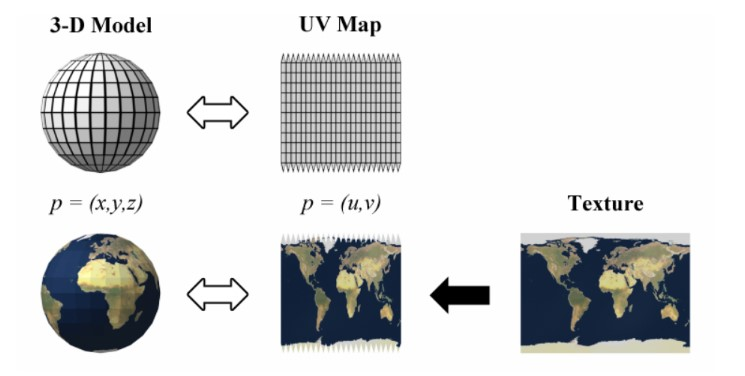
\includegraphics[scale=1]{sphere_uv_map.jpg}
    \caption{Normal para superfície curva do cone}
    \label{fig:sphere_uv_map}
  \end{figure}

  \label{code:sphere_texCoord}
  \begin{lstlisting}
    for (unsigned int slice = 1; slice <= slices; ++slice) {
        for (unsigned int stack = 1; stack <= stacks; ++stack) {
            auto fslice = (float) slice;
            auto fstack = (float) stack;

            vertices.emplace_back (r, theta + s * fslice, phi + t * fstack);
            texture.emplace_back (fslice / fslices, fstack / fstacks);
          }
    }
  \end{lstlisting}

\end{itemize}

\subsubsection{Cone}
\begin{figure}[H]
  \centering
  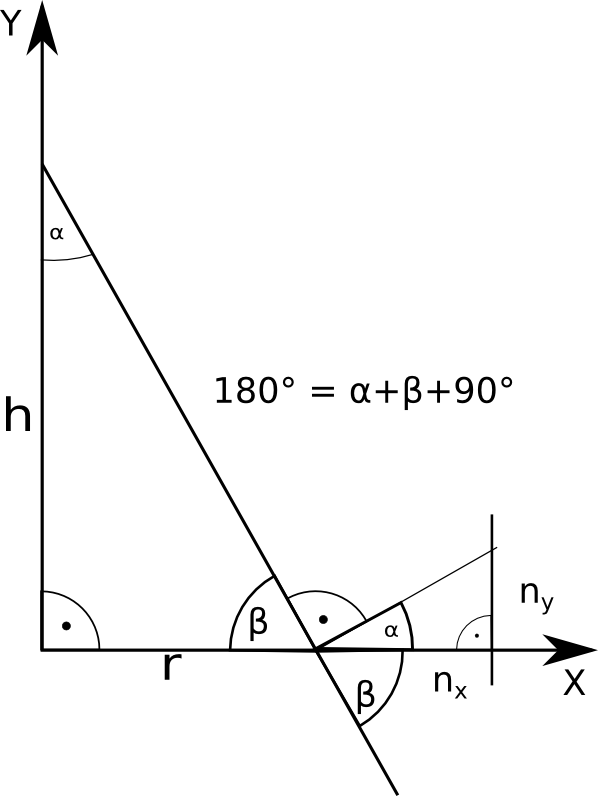
\includegraphics[scale=0.2]{cone_normal.png}
  \caption{Normal para superfície curva do cone}
  \label{fig:cone_normal}
\end{figure}

\begin{itemize}
  \item As normais do cone são calculadas de acordo com uma aproximação: para cada triângulo,
  calcula-se o seu vetor normal, que será dado a cada um dos seus vértices componentes.

  No entanto, os autores reconhecem que esta aproximação não se adequa para superfícies curvas
  como a do cone, servindo melhor para modelos que são intencionalmente poligonais.
  Devido à fórmula que se utilizou para o cálculo do cone (obtida, como referido em relatórios
  anteriores, através do serviço \url{https://www.math3d.org}), não foi possível adaptar facilmente a fórmula
  que se deriva da imagem ~\ref{fig:cone_normal}, que seria:

  $$
  (\cos(\beta) \cdot \sin(\alpha), \sin(\beta), \cos(\beta) \cdot \cos(\alpha) )
  $$

  \begin{lstlisting}
    beta = atan(radius / height);

    for (int st = 0; st <= stacks; st++) {
        for (int sl = 0; sl <= slices; sl++) {
            alpha = sl * alpha_offset;
    
            curr_x = new_radius * sin(alpha);
            curr_y = st * stack_height;
            curr_z = new_radius * cos(alpha);
    
            vertices.emplace_back(curr_x, curr_y, curr_z);
            textures.emplace_back( sl / (float) slices, st / (float) stacks);
            normals.emplace_back(
                cos(beta) * sin(alpha),
                sin(beta),
                cos(beta) * cos(alpha));
        }
      ...
    }
  \end{lstlisting}

\end{itemize}

\subsubsection{Superfície de Bezier}

\begin{itemize}
  \item As normais para as superfícies de Bezier foram simples, cortesia do Professor Ramires.

  \begin{figure}[H]
    \centering
    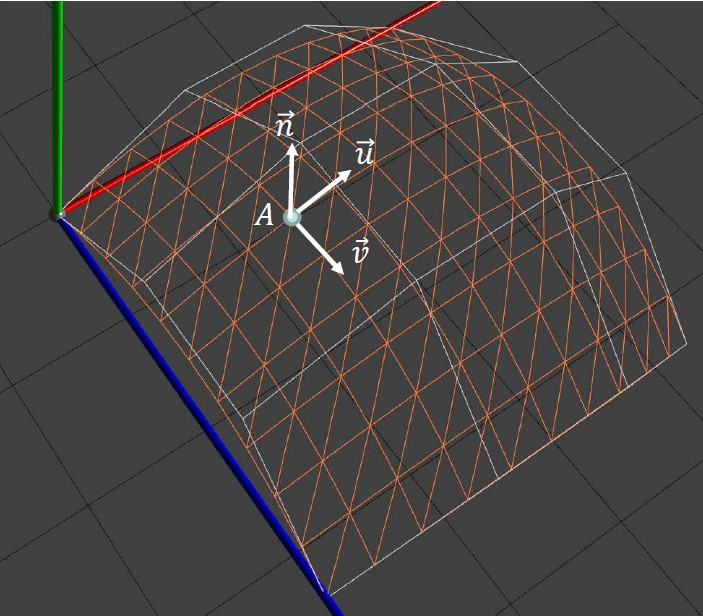
\includegraphics[scale=0.5]{bezier_normal.jpg}
    \caption{Normal para superfície de Bezier}
    \label{fig:bezier_normal}
  \end{figure}

  \begin{figure}[H]
    \centering
    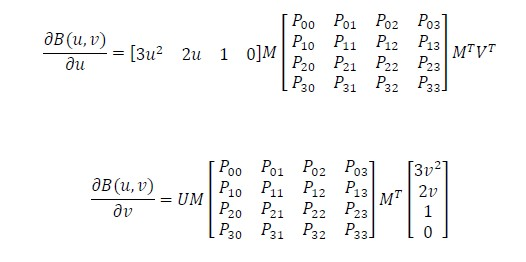
\includegraphics[scale=1]{bezier_normal_2.jpg}
    \caption{Cálculo de normal para superfície de Bezier}
    \label{fig:bezier_normal_2}
  \end{figure}

  Nota-se apenas que o cálculo em~\ref{fig:bezier_normal_2} foi relativamente simplificado por se ter usado a
  biblioteca \texttt{glm}\footnote{código fonte em \url{https://github.com/g-truc/glm}}.

  \item Para as texturas: considere-se o exemplo dado pelo Professor:
  
  \begin{figure}[H]
    \centering
    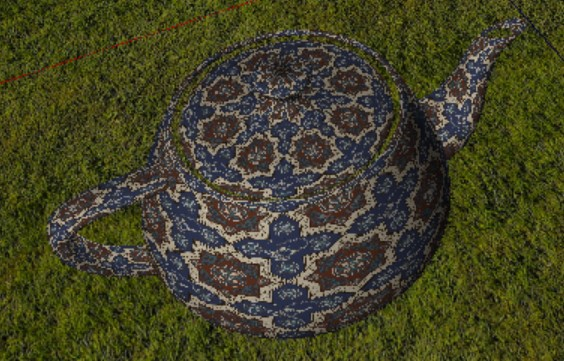
\includegraphics[scale=1]{bezier_texture.jpg}
    \caption{Exemplo de superfície de Bezier com textura}
    \label{fig:bezier_texture}
  \end{figure}

  Para obter este efeito com repetições, fez-se o seguinte código:

  \begin{lstlisting}
    auto float_tesselation = (float) int_tesselation;
    const auto step = 1.0 / float_tesselation;
    
    for (int v = 0; v < int_tesselation; ++v) {
        for (int u = 0; u < int_tesselation; ++u) {
            get_bezier_point_at (
              u * step,
              v * step,
              control_points,
              vertex,
              normal);
    
            auto fu = (float) u;
            auto fv = (float) v;
            vec3 vertex, normal;
            vertices.push_back (vertex);
            normals.push_back (normal);
            texture.emplace_back (-(u * step), -(v * step));
        }
    }
  \end{lstlisting}

  ou seja, está-se a repetir a textura ao longo dos ``\textit{patches}'' da superfície.

\end{itemize}

\newpage

\section{\texttt{Engine.cpp}}

Para poder lidar com os novos campos XML com informação sobre luzes, propriedades dos
materiais e ficheiros de textura, o código de ``\textit{parsing}'' em \texttt{parsing.cpp}
descrito nos relatórios anteriores teve que ser atualizado.

\subsection{Valores por defeito para as luzes}

Como não foi definido no enunciado que valores de RGB utilizar para as diferentes componentes
de luz que o OpenGL suporta, escolheram-se os seguintes:

\begin{lstlisting}
const auto RGB_MAX = 255.0;
struct model {
  GLsizei nVertices{};
  GLuint vbo{};
  GLuint normals{};
  struct {
/*
Source:
https://www.khronos.org/registry/OpenGL-Refpages/gl2.1/xhtml/glMaterial.xml
*/
    vec4 diffuse{200.0 / RGB_MAX, 200.0 / RGB_MAX, 200.0 / RGB_MAX, 1};
    vec4 ambient{50.0 / RGB_MAX, 50.0 / RGB_MAX, 50.0 / RGB_MAX, 1};
    vec4 specular{0, 0, 0, 1};
    vec4 emissive{0, 0, 0, 1};
    GLfloat shininess = 0;
  } material{};
/*
0 default value means it's optional with 0 meaning
it's not being used by a particular model.
*/
  GLuint tbo = 0; // texture buffer object
  GLuint tc = 0; // texture coordinates
};
\end{lstlisting}


\chapter{Trabalho adicional} \label{chap:plus} %referência cruzada

\section{Extensão ao XML}

De forma a poder executar os testes mais rapidamente, efetuaram-se mudanças no \texttt{engine}
para poder aceitar ficheiros XML com as seguintes modificações:

\lstset{language=XML,
  basicstyle=\small, % print whole listing small
  keywordstyle=\color{cyan}\bfseries\underbar,
  % underlined bold black keywords
  identifierstyle={\color{blue}},%
  commentstyle=\color{purple}, % brown comments
  showstringspaces=true,
  % Without this it is not possible to have bash dollar signs inside \lstlisting.
  escapeinside=||,
  morekeywords={group, models, model, generator, argv, texture, file}
}
\begin{lstlisting}
  <group>
      <models>
          <model file="plane.3d"> <!-- generator plane 1 3 plane_nt.3d -->
              <generator argv="plane 2 1 plane.3d"/>
              <texture file="../test_files_phase_4/relva.jpg"/>
          </model>
      </models>
  </group>
\end{lstlisting}

Através do uso do padrão \texttt{fork() / exec()}, e tornando o executável \texttt{engine}
dependente do \texttt{generator} no \texttt{cmake}, simplifica-se a compilação e execução de um cenário
de teste.
\\

\texttt{./engine test\_4\_7.xml}, contendo toda a informação necessária para correr \texttt{generator},
gerará os vértices, normais e coordenadas de textura para cada modelo no ficheiro, e iniciará o programa
com os ficheiros ``.3d'' necessários.

Veja-se o exemplo completo no Anexo~\ref{code:extended_xml}

\section{Câmara FPS}

Implementou-se, para além do modo explorador fornecido pelo Professor Ramires
para as aulas práticas, um modo FPS com movimento através de periféricos (rato/teclado) para exploração
do sistema solar.\\

É possível alterar os dois modos dinamicamente durante a execução do programa.

\section{``\textit{Skybox}'' para sistema solar}

Por sugestão do Professor Carlos Brito, para simular um ambiente visual mais rico durante a execução
do \texttt{engine} com o modelo do sistema solar, acrescentou-se uma ``\textit{skybox}'' com uma textura
apropriada, retirada de \href{https://svs.gsfc.nasa.gov/4851}{Deep Star Maps 2020}.

O método é o seguinte:

\begin{itemize}
  \item Acrescenta-se uma esfera com tamanho apropriado no XML do sistema solar.
  \item Escolhe-se a textura que cobrirá o modelo da esfera
  \item Trata-se o modelo como todos os outros a respeito de textura, e ``\textit{rendering}''.
\end{itemize}

\begin{figure}[H]
  \centering
  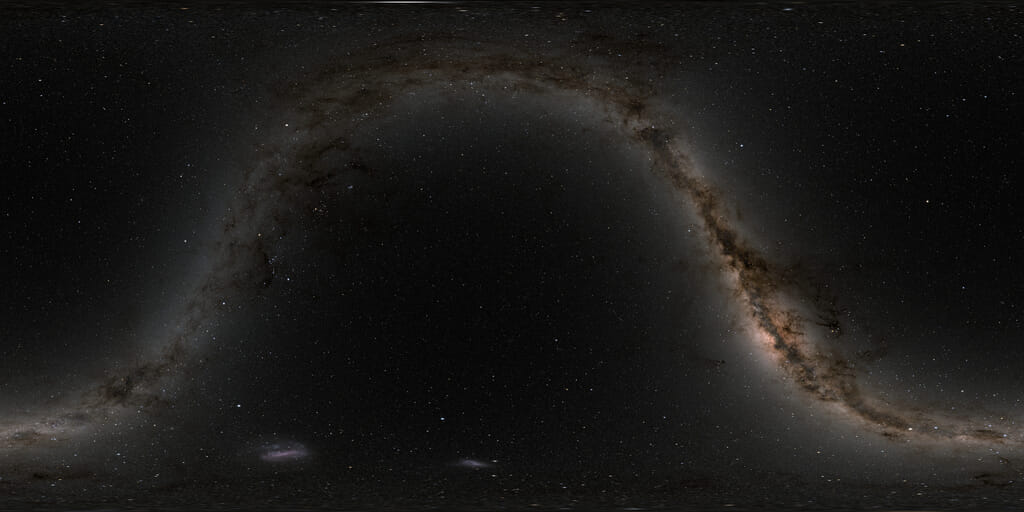
\includegraphics[scale=0.4]{galaxy.jpg}
  \caption{Imagem utilizada para pano de fundo}
  \label{fig:galaxy}
\end{figure}

\section{Movimento no espaço através de periférico}

Através da função \href{https://www.khronos.org/registry/OpenGL-Refpages/gl2.1/xhtml/gluUnProject.xml}{\texttt{glUnProject}},
é possível, através de ``\textit{input}'' predefinido (neste caso, o botão direito do rato), movimentar a posição
da câmara no espaço global para a posição do cursor na janela.

\chapter{Exemplo de utilização} \label{chap:exemps} %referência cruzada

Observe-se na imagem abaixo o sistema solar, com a ``\textit{skybox}'' escolhida, assim como
o ``cometa'' com trajetória numa curva de Catmull-Rom.

\begin{figure}[H]
  \centering
  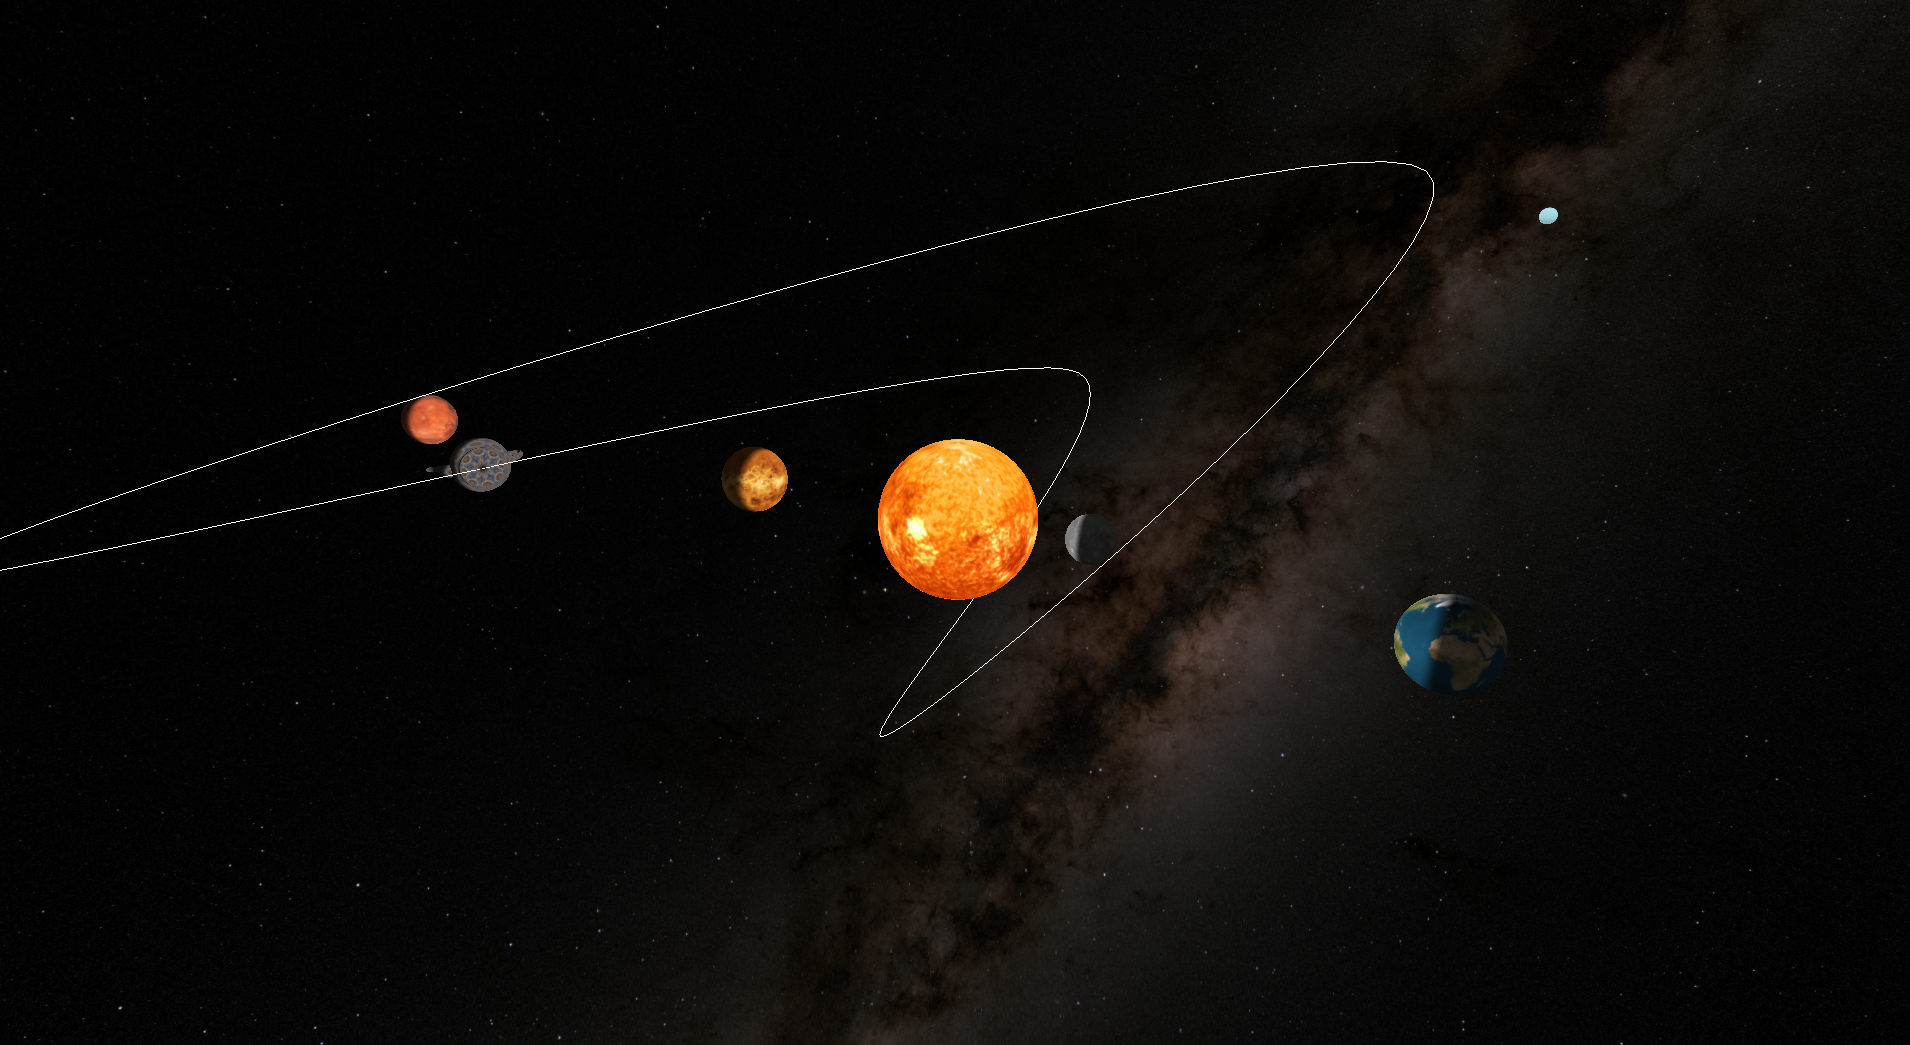
\includegraphics[scale=0.4]{exemplo.png}
  \caption{Sistema solar com órbita de ecometa e Via Lácter visíveis}
  \label{fig:exemplo}
\end{figure}

\chapter{Conclusão} \label{concl}

Conclui-se desta forma a apresentação da fase 4 do Projeto Prático de \cg do Grupo 3.

\section{Comentários}

A aproximação que se utilizou ao gerar as normais de superfície do cone, embora
produza efeitos aceitáveis, não é ideal porque se o número de ``\textit{slices}'' for baixo,
terá precisão baixa quando comparada com a utilização da fórmula correta.

\section{Trabalho Futuro}

Este projeto foi escrito num contexto académico, e não terá qualquer uso futuro adicional.\\

Se tivesse, a primeira necessidade seria alterar a geração dos modelos de sólidos geométricos
para facilitar o cálculo de normais e coordenadas de textura - embora o serviço Math3d tenha
auxiliado na fase inicial para prototipagem, dificultou, no final, o cálculo dessa componentes
para cada modelos.

\appendix % apendice
\chapter{Excertos de Código Utilizado no Projeto}

\lstset{language=XML,
  basicstyle=\small, % print whole listing small
  keywordstyle=\color{cyan}\bfseries\underbar,
  % underlined bold black keywords
  identifierstyle={\color{blue}},%
  commentstyle=\color{purple}, % brown comments
  showstringspaces=true,
  % Without this it is not possible to have bash dollar signs inside \lstlisting.
  escapeinside=||,
  morekeywords={
    world, dir, group, models, model, generator, argv, texture, file,
    specular, ambient, diffuse, emissive, lights, light,
    transform, translate, rotate, scale,
    type, camera}
}

\label{code:extended_xml}
\begin{lstlisting}[caption={Exemplo de XML com informação adicional de geração de modelos}]
  <world>
  <generator dir="../bin/generator"/>
  <camera>
      <position x="-0.740200" y="1.182951" z="1.376347"/>
      <lookAt x="0" y="0" z="0"/>
      <up x="0" y="1" z="0"/>
      <projection fov="60" near="1" far="1000"/>
  </camera>

  <lights>
      <light type="point" posX="0" posY="0.2" posZ="0"/>
      <light type="point" posX="-2" posY="2" posZ="2"/>
      <!--        <light type="directional" dirX="-2" dirY="2" dirZ="2"/>-->
  </lights>

  <group>
      <group>
          <models>
              <model file="plane.3d"> <!-- generator plane 1 3 plane_nt.3d -->
                  <generator argv="plane 2 1 plane.3d"/>
                  <texture file="../test_files_phase_4/relva.jpg"/>
              </model>
          </models>
      </group>
      <group>
          <transform>
              <translate x="-0.5" y="0" z="-0.5"/>
              <scale x="0.2" y="0.2" z="0.2"/>
          </transform>
          <models>
              <model file="cone.3d"> <!-- generator cone 1 2 10 10 cone_nt.3d -->
                  <generator argv="cone 1 2 5000 100 cone.3d"/>
                  <texture file="../test_files_phase_4/cone.jpg"/>
              </model>
          </models>
      </group>
      <group>
          <transform>
              <translate x="0.5" y="0.2" z="0.5"/>
              <scale x="0.2" y="0.2" z="0.2"/>
          </transform>
          <models>
              <model file="sphere.3d"> <!-- generator sphere 1 32 32 sphere_nt.3d -->
                  <generator argv="sphere 1 100 100 sphere.3d"/>
                  <texture file="../test_files_phase_4/earth.jpg"/>
              </model>
          </models>
      </group>
      <group>
          <transform>
              <translate x="-0.5" y="0" z="0.5"/>
              <scale x="0.1" y="0.1" z="0.1"/>
              <rotate angle="-90" x="1" y="0" z="0"/>
          </transform>
          <models>
              <model file="teapot.3d"> <!-- generator patch teapot.patch 10 bezier_nt.3d -->
                  <generator argv="bezier ../test_files_phase_3/teapot.patch 10 teapot.3d"/>
                  <texture file="../test_files_phase_4/teapot.jpg"/>
              </model>
          </models>
      </group>
      <group>
          <transform>
              <scale x="0.2" y="0.2" z="0.2"/>
              <translate x="2.5" y="1.0" z="-2.5"/>
          </transform>
          <models>
              <model file="box.3d"> <!-- generator box 2 3 box_nt.3d -->
                  <generator argv="box 2 3 box.3d"/>
                  <texture file="../test_files_phase_4/box.jpg"/>
              </model>
          </models>
      </group>

  </group>
</world>
\end{lstlisting}

\newpage

%-- Fim do documento -- inserção das referencias bibliográficas

%\bibliographystyle{plain} % [1] Numérico pela ordem de citação ou ordem alfabetica
\bibliographystyle{alpha} % [Hen18] abreviação do apelido e data da publicação
%\bibliographystyle{apalike} % (Araujo, 2018) apelido e data da publicação
                             % --para usar este estilo descomente no inicio o comando \usepackage{apalike}

\bibliography{bibLayout} %input do ficheiro de referencias bibliograficas

\end{document}